% Options for packages loaded elsewhere
\PassOptionsToPackage{unicode,pdfusetitle}{hyperref}
\PassOptionsToPackage{hyphens}{url}
\PassOptionsToPackage{dvipsnames,svgnames*,x11names*}{xcolor}

\documentclass[10pt,ignorenonframetext]{beamer}
\usepackage{lmodern}
\usepackage{amssymb,amsmath,mathtools,amsthm}
\usepackage[T1]{fontenc}
\usepackage[utf8]{inputenc}
\usepackage{textcomp} % provide euro and other symbols

\usepackage{pgfpages}

% prevent slide breaks in the middle of a paragraph
\widowpenalties 1 10000
\raggedbottom

% redefine part, section, and subsection headers
\raggedbottom
\setbeamertemplate{part page}{
 \centering
 \begin{beamercolorbox}[sep=16pt,center]{part title}
    \usebeamerfont{part title}\insertpart\par
 \end{beamercolorbox}
}
\setbeamertemplate{section page}{
 \centering
 \begin{beamercolorbox}[sep=12pt,center]{part title}
    \usebeamerfont{section title}\insertsection\par
 \end{beamercolorbox}
}
\setbeamertemplate{subsection page}{
 \centering
 \begin{beamercolorbox}[sep=8pt,center]{part title}
    \usebeamerfont{subsection title}\insertsubsection\par
 \end{beamercolorbox}
}

\AtBeginPart{\frame{\partpage}}
\AtBeginSection{\ifbibliography\else\frame{\sectionpage}\fi}
\AtBeginSubsection{\frame{\subsectionpage}}

% beamer configuration
\usecolortheme{dove}
\usefonttheme{professionalfonts}
\usefonttheme{structurebold}

\setbeamertemplate{footline}[frame number]

\setbeamertemplate{caption}[numbered]
\setbeamertemplate{caption label separator}{: }
\setbeamercolor{caption name}{fg=normal text.fg}

\setbeamertemplate{frametitle}{\begin{centering}\insertframetitle\par\end{centering}\medskip}

\setbeamertemplate{itemize item}{$\bullet$}
%\setbeamertemplate{itemize item}[circle]
\setbeamertemplate{itemize subitem}{$\circ$}
\setbeamertemplate{itemize subsubitem}{\textendash}
\setbeamerfont{frametitle}{size=\large}
\setbeamertemplate{headline}{\vskip6ex}
\beamertemplatenavigationsymbolsempty
%\setlength{\parskip}{1em} % add paragraph spacing

% Use upquote if available, for straight quotes in verbatim environments
\usepackage{upquote}
\usepackage[]{microtype}
\UseMicrotypeSet[protrusion]{basicmath} % disable protrusion for tt fonts

\usepackage{xcolor}
\usepackage{xurl} % add URL line breaks if available
\usepackage{bookmark}
\usepackage{hyperref}
\hypersetup{
  colorlinks=false,
  linkcolor=Maroon,
  filecolor=Maroon,
  citecolor=Blue,
  urlcolor=Blue
}

% tikz and pgfplots stuff
\usepackage{tikz}
\usetikzlibrary{arrows,shapes,positioning,intersections,backgrounds}
\usepackage{pgfplots}
\usepgfplotslibrary{external,colormaps}
\pgfplotsset{width=5cm,compat=1.16}
%\tikzexternalize

% misc
\urlstyle{same} % disable monospaced font for URLs
\newif\ifbibliography
\setlength{\emergencystretch}{3em} % prevent overfull lines
\setcounter{secnumdepth}{-\maxdimen} % remove section numbering
\usepackage{subcaption}
\usepackage{booktabs}

% algorithms
\usepackage{algorithm,algpseudocode}
%\algblockdefx{Repeat}{EndRepeat}{\textbf{repeat}}{}
%\algnotext{EndRepeat}

% operators
\DeclareMathOperator*{\argmax}{arg\,max}
\DeclareMathOperator*{\argmin}{arg\,min}
\DeclareMathOperator{\E}{\text{E}}
\DeclareMathOperator{\var}{var}
\DeclareMathOperator{\cov}{cov}
\DeclareMathOperator{\sign}{sign}
\DeclareMathOperator{\card}{card}
\DeclareMathOperator{\cumsum}{cumsum}
\DeclareMathOperator*{\prox}{prox}

% macros
\newcommand{\pkg}[1]{\textsf{#1}}
\renewcommand{\vec}{\vectorsym}
\newcommand{\mat}{\matrixsym}
\newcommand{\du}{\mathrm{d}}

% biblatex
%\usepackage[citestyle=authoryear]{biblatex}
%\addbibresource{references.bib}

\title{Pathwise Coordinate Descent}
\subtitle{Presentation for PhD Group}
\author{Johan Larsson}
\date{\today}
\institute{Department of Statistics, Lund University}
\titlegraphic{\includegraphics{lu.pdf}}

\begin{document}
\frame[noframenumbering,plain]{\titlepage}

\begin{frame}{Overview}
\tableofcontents
\end{frame}

\section{Coordinate Descent}

\begin{frame}{Setting}

The general problem we want to solve is
\[
\operatorname*{minimize}_{x \in \mathbb{R}^p} f(x),
\]
with \(f : \mathbb{R}^p \mapsto \mathbb{R}\) convex and continuous.

\begin{figure}
    \centering
    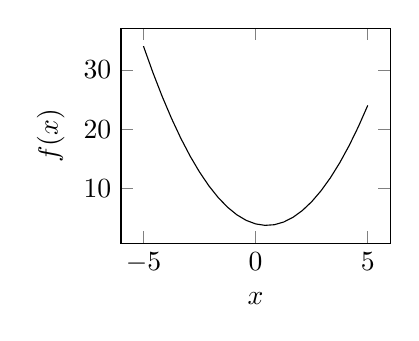
\begin{tikzpicture}
	\begin{axis}[
		xlabel=$x$,
		ylabel={$f(x)$}
	]
	% use TeX as calculator:
	\addplot[black,mark=none]{x^2 - x +4};
	\end{axis}
    \end{tikzpicture}
\end{figure}

\alert{standard methods:} gradient descent, Newton's method, etc.

\end{frame}

\begin{frame}{Coordinate Descent}
    The (very simple) idea of coordinate descent is to minimize \(f(x)\) \alert{one coordinate (variable) at the time}.
    \begin{algorithm}[H]
        \caption{Coordinate Descent}
        \begin{algorithmic}
        \While{stopping criterion not reached}
        \State pick coordinate \(j\) from \(\{1,2,\dots,p\}\)
        \State \(x_j \gets \argmin_{x_j \in \mathbb{R}} f(x)\)
        \EndWhile
        \end{algorithmic}
    \end{algorithm}
    
    \alert{Important:} always use most recent coordinate update
\end{frame}

\begin{frame}{Convex and Differentiable}

For \(f(x)\) \alert{convex} and \alert{differentiable}, CD always obtains the global minimum.

\begin{figure}
    \centering
    \includegraphics{figures/cd-convex-differentiable.pdf}
    \caption{Coordinate descent for \(f(x_1,x_2) = 5x_1^2 - 6x_1x_2 + 5x_2^2\).}
\end{figure}

\end{frame}

\begin{frame}{Convex and Non-Differentiable}

For \alert{non-differentiable} \(f\), however, the algorithm need not converge.

\begin{figure}
    \centering
    \includegraphics{figures/cd-non-differentiable.pdf}
    \caption{Coordinate descent for \(f(x_1,x_2) = |x + y| + 3|x-y|\).}
\end{figure}
\end{frame}

\begin{frame}{Convex, Non-Differentiable, but Separable}

It turns out that if \(f\) is of the form \[f(x) = g(x) + \sum_{j=1}^p h(x_j),\] i.e. \alert{separable}, then the algorithm converges even if each \(h_j\) is non-differentiable.

\medskip

\pause

Why does this matter? Because many useful penalties have exactly this form!
\begin{itemize}
    \item lasso (and elastic net)
    \item the nonnegative garotte
    \item LAD-lasso
    \item group lasso
\end{itemize}
\end{frame}

\section{The Lasso}

\begin{frame}{The Lasso}

The lasso solves the following problem:
\[
\begin{aligned}
&\text{minimize} && \frac 12 \sum_{i=1}^n \left( y_i - \sum_{j=1}^p x_{ij}\beta_j \right)^2\\
& \text{subject to} && \sum_{j=1}^p |\beta_j| \leq t.
\end{aligned}
\]


\begin{columns}
\begin{column}{0.45\linewidth}
    \(t\) is kind of a \alert{budget} on the magnitude of the coefficient vector.
\end{column}
\begin{column}{0.45\linewidth}
    \begin{figure}
        \centering
        \pgfplotsset{width=6cm,height=6cm}
        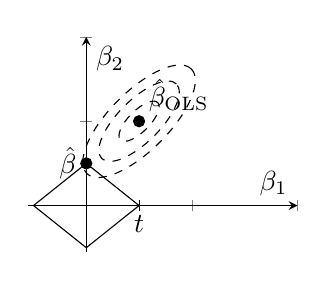
\begin{tikzpicture}
\begin{axis}[
    xlabel = \(\beta_1\),
    ylabel = \(\beta_2\),
    ymin = -1.1,
    ymax = 4,
    xmin = -1.1,
    xmax = 4,
    axis lines = center,
    yticklabels={,,},
    xticklabels={,,}
]
\draw[dashed, rotate around={45:(1,2)}] (1,2) ellipse (0.5 and 0.25);
\draw[dashed, rotate around={45:(1,2)}] (1,2) ellipse (1 and 0.5);
\draw[dashed, rotate around={45:(1,2)}] (1,2) ellipse (1.4 and 0.7);

\addplot[]
    coordinates {
    	(-1,0)
    	(0,1)
    	(1,0)
    	(0,-1)
    	(-1,0)
    };
    
\addplot [only marks, mark=*] coordinates {(1,2)};
\node [above right,black] at (1,2) {\(\hat\beta_\text{OLS}\)};

\addplot [only marks, mark=*] coordinates { (0,1) };
\node [left] at (0,1) {$\hat\beta$};

\addplot [only marks, mark = |] coordinates { (1, 0) };
\node [below] at (1,0) {\(t\)};
\end{axis}
\end{tikzpicture}
    \end{figure}
\end{column}
\end{columns}
\end{frame}

\begin{frame}{Lasso in Lagrangian form}
To solve the lasso, we typically transform it into an \alert{unconstrained} optimization problem:
\[
\text{minimize} \quad \frac 12 \sum_{i=1}^n \left( y_i - \sum_{j=1}^p x_{ij}\beta_j \right)^2 + \lambda \sum_{j=1}^p |\beta_j|.
\]
high values of \(\lambda\): strong penalization, sparse solutions

\pause

\begin{block}{Regularization Path}
usually don't know \(\lambda\) in advance

\medskip

typically select it using \alert{grid search} (with cross-validation): start at large \(\lambda\); finish at small \(\lambda\) (OLS)

\end{block}
\end{frame}

\begin{frame}{The Lasso Path}
\begin{figure}
    \centering
    \includegraphics{figures/lasso-path.pdf}
\end{figure}
\end{frame}

\begin{frame}{Coordinate Descent for the Lasso: One Predictor}

Assume \(x\) standardized, then the problem reduces to 
\[
\text{minimize}_\beta \quad \frac 12 \left(\beta - \hat\beta_\mathrm{OLS}\right)^2 + \lambda |\beta|,
\]
leading to \[ \hat\beta_\mathrm{lasso} = \operatorname{S}(\hat\beta_\mathrm{OLS}; \lambda) = \sign(\hat\beta_\mathrm{OLS})\left(|\hat\beta_\mathrm{OLS}| - \lambda\right)_+.\]

\(\operatorname{S}(\cdot; \lambda)\) is the \alert{soft-thresholding} operator.

\begin{figure}
    \centering
    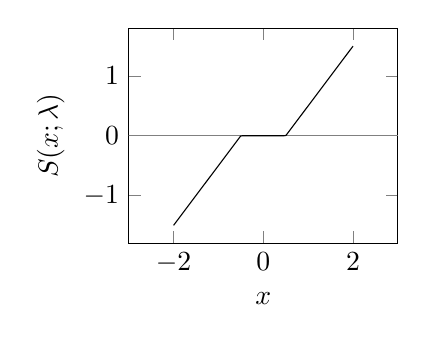
\begin{tikzpicture}
\begin{axis}[xlabel={$x$}, ylabel={$S(x;\lambda)$}, xmin={-3}, xmax={3}]
    \addplot[no marks, gray]
        {0.0};
    \addplot[no marks]
        coordinates {
            (-2.0,-1.5)
            (-1.9595959595959596,-1.4595959595959596)
            (-1.9191919191919191,-1.4191919191919191)
            (-1.878787878787879,-1.378787878787879)
            (-1.8383838383838385,-1.3383838383838385)
            (-1.797979797979798,-1.297979797979798)
            (-1.7575757575757576,-1.2575757575757576)
            (-1.7171717171717171,-1.2171717171717171)
            (-1.6767676767676767,-1.1767676767676767)
            (-1.6363636363636365,-1.1363636363636365)
            (-1.595959595959596,-1.095959595959596)
            (-1.5555555555555556,-1.0555555555555556)
            (-1.5151515151515151,-1.0151515151515151)
            (-1.4747474747474747,-0.9747474747474747)
            (-1.4343434343434343,-0.9343434343434343)
            (-1.393939393939394,-0.893939393939394)
            (-1.3535353535353536,-0.8535353535353536)
            (-1.3131313131313131,-0.8131313131313131)
            (-1.2727272727272727,-0.7727272727272727)
            (-1.2323232323232323,-0.7323232323232323)
            (-1.1919191919191918,-0.6919191919191918)
            (-1.1515151515151516,-0.6515151515151516)
            (-1.1111111111111112,-0.6111111111111112)
            (-1.0707070707070707,-0.5707070707070707)
            (-1.0303030303030303,-0.5303030303030303)
            (-0.98989898989899,-0.48989898989898994)
            (-0.9494949494949495,-0.4494949494949495)
            (-0.9090909090909091,-0.40909090909090906)
            (-0.8686868686868687,-0.36868686868686873)
            (-0.8282828282828283,-0.3282828282828283)
            (-0.7878787878787878,-0.28787878787878785)
            (-0.7474747474747475,-0.24747474747474751)
            (-0.7070707070707071,-0.20707070707070707)
            (-0.6666666666666666,-0.16666666666666663)
            (-0.6262626262626263,-0.1262626262626263)
            (-0.5858585858585859,-0.08585858585858586)
            (-0.5454545454545454,-0.045454545454545414)
            (-0.5050505050505051,-0.005050505050505083)
            (-0.46464646464646464,-0.0)
            (-0.42424242424242425,-0.0)
            (-0.3838383838383838,-0.0)
            (-0.3434343434343434,-0.0)
            (-0.30303030303030304,-0.0)
            (-0.26262626262626265,-0.0)
            (-0.2222222222222222,-0.0)
            (-0.18181818181818182,-0.0)
            (-0.1414141414141414,-0.0)
            (-0.10101010101010101,-0.0)
            (-0.06060606060606061,-0.0)
            (-0.020202020202020204,-0.0)
            (0.020202020202020204,0.0)
            (0.06060606060606061,0.0)
            (0.10101010101010101,0.0)
            (0.1414141414141414,0.0)
            (0.18181818181818182,0.0)
            (0.2222222222222222,0.0)
            (0.26262626262626265,0.0)
            (0.30303030303030304,0.0)
            (0.3434343434343434,0.0)
            (0.3838383838383838,0.0)
            (0.42424242424242425,0.0)
            (0.46464646464646464,0.0)
            (0.5050505050505051,0.005050505050505083)
            (0.5454545454545454,0.045454545454545414)
            (0.5858585858585859,0.08585858585858586)
            (0.6262626262626263,0.1262626262626263)
            (0.6666666666666666,0.16666666666666663)
            (0.7070707070707071,0.20707070707070707)
            (0.7474747474747475,0.24747474747474751)
            (0.7878787878787878,0.28787878787878785)
            (0.8282828282828283,0.3282828282828283)
            (0.8686868686868687,0.36868686868686873)
            (0.9090909090909091,0.40909090909090906)
            (0.9494949494949495,0.4494949494949495)
            (0.98989898989899,0.48989898989898994)
            (1.0303030303030303,0.5303030303030303)
            (1.0707070707070707,0.5707070707070707)
            (1.1111111111111112,0.6111111111111112)
            (1.1515151515151516,0.6515151515151516)
            (1.1919191919191918,0.6919191919191918)
            (1.2323232323232323,0.7323232323232323)
            (1.2727272727272727,0.7727272727272727)
            (1.3131313131313131,0.8131313131313131)
            (1.3535353535353536,0.8535353535353536)
            (1.393939393939394,0.893939393939394)
            (1.4343434343434343,0.9343434343434343)
            (1.4747474747474747,0.9747474747474747)
            (1.5151515151515151,1.0151515151515151)
            (1.5555555555555556,1.0555555555555556)
            (1.595959595959596,1.095959595959596)
            (1.6363636363636365,1.1363636363636365)
            (1.6767676767676767,1.1767676767676767)
            (1.7171717171717171,1.2171717171717171)
            (1.7575757575757576,1.2575757575757576)
            (1.797979797979798,1.297979797979798)
            (1.8383838383838385,1.3383838383838385)
            (1.878787878787879,1.378787878787879)
            (1.9191919191919191,1.4191919191919191)
            (1.9595959595959596,1.4595959595959596)
            (2.0,1.5)
        }
        ;
\end{axis}
\end{tikzpicture}

\end{figure}

\end{frame}

\begin{frame}

\begin{figure}
    \centering
    \includegraphics[width=0.85\linewidth]{figures/lasso-single-predictor.pdf}
    \caption{The solution to two lasso problems with one predictor each. The dashed line marks the (unpenalized) ordinary least-squares solution. The red line marks the lasso solution. (\(\gamma \coloneqq \lambda\) in our notation.)}
\end{figure}
    
\end{frame}

\begin{frame}{Coordinate Descent for the Lasso: Several Predictors}

Rewrite lasso objective as 
\[
f(\beta) = \frac 12 \sum_{i=1}^n\left(y_i - \sum_{k \neq j}x_{ik}\beta_k - x_{ij}\beta_j\right)^2 + \lambda \sum_{k \neq j}|\beta_k| + \lambda | \beta_j|,
\]
hold \(\beta_k\) for \(k \neq j\) fixed, and minimize with respect to \(\beta_j\):
\[
\argmin_{\beta_j \in \mathbb{R}} f(\beta) = \operatorname{S}\left( \sum_{i=1}^n x_{ij}\bigg(y_i - \sum_{k \neq j} x_{ik}\beta_k\bigg); \lambda\right)
\]
\medskip
\alert{Key}: updates are cheap!
    
\end{frame}

\begin{frame}{Convergence}

\begin{figure}
    \centering
    \includegraphics[width=0.6\linewidth]{figures/cd-convergence.png}
    \caption{Coordinate descent and proximal gradient for lasso with \(n = 200\), \(p=50\).}
\end{figure}
    
\end{frame}

\section{The Fused Lasso}

\begin{frame}{The Fused Lasso}

The Fused Lasso minimizes
\[
\frac 12 \sum_{i=1}^n \left( y_i - \sum_{j=1}^px_{ij}\beta_j\right)^2 + \lambda_1 \sum_{j=1}^p|\beta_j| + \lambda_j \sum_{j=2}^p |\beta_j - \beta_{j-1}|.
\]

\begin{figure}
    \centering
    \pgfplotsset{width=6cm,height=6cm}
    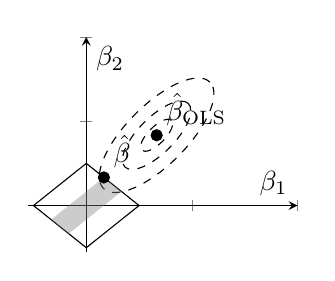
\begin{tikzpicture}
    \begin{axis}[
        xlabel = \(\beta_1\),
        ylabel = \(\beta_2\),
        ymin = -1.1,
        ymax = 4,
        xmin = -1.1,
        xmax = 4,
        axis lines = center,
        yticklabels={,,},
        xticklabels={,,}
    ]
        \draw[dashed, rotate around={45:(1.333,1.667)}] (1.333,1.667) ellipse (0.4 and 0.2);
        \draw[dashed, rotate around={45:(1.333,1.667)}] (1.333,1.667) ellipse (0.85 and 0.425);
        \draw[dashed, rotate around={45:(1.333,1.667)}] (1.333,1.667) ellipse (1.425 and 0.7125);
        
        \addplot [only marks, mark=*] coordinates {(1.333,1.667)};
        \node [above right,black] at (1.333,1.667) {\(\hat\beta_\text{OLS}\)};
        
        \addplot[]
            coordinates {
            	(-1,0)
            	(0,1)
            	(1,0)
            	(0,-1)
            	(-1,0)
            };
            
        \addplot[fill = gray, draw = none, opacity = 0.4]
            coordinates {
                (-2/3, -1/3)
                (-1/3, -2/3)
                (2/3, 1/3)
                (1/3, 2/3)
            };
        
        \addplot [only marks, mark=*] coordinates { (1/3,2/3) };
        \node [above right] at (1/3,2/3) {$\hat\beta$};
    \end{axis}
\end{tikzpicture}
\end{figure}

\end{frame}


\begin{frame}{Standard CD Does not Work for the Fused Lasso}

The fused lasso penalty, however, isn't \alert{separable}, which means that convergence is no longer guaranteed!

\begin{figure}
    \centering
    \includegraphics[width=\linewidth]{figures/fused-lasso-failure.png}
    \caption{Coordinate descent failure for fused lasso problem.}
\end{figure}

\end{frame}


\begin{frame}{FLSA}

We begin with a special case of the fused lasso: the fused lasso signal approximator (FLSA):
\[
\operatorname*{minimize}_\beta \left\{ \frac 12 \sum_{i=1}^n(y_i - \beta_i)^2 + \lambda_1 \sum_{i=1}^n|\beta_i| + \lambda_2 \sum_{i=2}^n |\beta_i - \beta_{i=1}|\right\}
\]

\begin{figure}
    \centering
    \includegraphics[width=\linewidth]{figures/fused-lasso-illustration.png}
    \caption{Fused lasso solution for signal approximation.}
\end{figure}
    
\end{frame}

\begin{frame}{Solving FLSA via Three Cycles}

\begin{block}{Descent cycle}
    run coordinate descent for each \(\beta_j\)
\end{block}

\begin{block}{Fusion cycle}
    consider fusing neighboring parameters
\end{block}

\begin{algorithm}[H]
\caption{CD for the fused lasso (smoothing cycle).}
    \begin{algorithmic}
        \Require \(\delta > 0\)
        \State \(\lambda_2 \gets 0\)
        \Repeat 
            \State \(\lambda_2 \gets \lambda_2 + \delta\)
            \Repeat 
                \State run \emph{descent cycle}
                \State run \emph{fusion cycle}
            \Until{no changes in coefficient estimates occur}
        \Until{until \(\lambda_2\) reaches target value}
    \end{algorithmic}
\end{algorithm}
\end{frame}

\begin{frame}{Descent Cycle}
Assume that \(\beta_i \notin \{0, \beta_{i-1}, \beta_{i+1}\}\), hold all \(\beta_k\), \(k \neq i\) fixed. Then,
\[
\frac{\partial f(\beta)}{\partial \beta_i} = -(y_i - \beta_i) + \lambda_1 \sign(\beta_i) - \lambda_2 \sign(\beta_{i+1} - \beta_i) + \lambda_2 \sign(\beta_i - \beta_{i-1}),
\]
which is \alert{piecewise linear}. \pause Then proceed to

\begin{enumerate}
    \item check for a zero in each interval
    \item if no zero is found, examine objective values at \(\beta_i = 0, \beta_{i-1}, \beta_{i+1}\)
\end{enumerate}

\begin{figure}
    \centering
    \includegraphics[width=\linewidth]{figures/fused-cd-cycles.png}
    %\caption{Caption}
\end{figure}
\end{frame}

\begin{frame}{Fusion Cycle}
Descent cycle can get stuck! The fusion cycle considers fusing \alert{two} coefficients and moving them together.\medskip

Enforce \(|\beta_i - \beta_{i-1}| = 0\) by letting \(\gamma \coloneqq \beta_i = \beta_{i=1}\) and minimize with respect to \(\gamma\).
\[
\begin{aligned}
\frac{\partial f(\beta)}{\partial \gamma} &= (-y_{i-1} - \gamma) - (y_i - \gamma) \\
&+ 2\gamma_1 \sign(\gamma) - \gamma_2 \sign(\beta_{i+1} - \gamma) \\ 
&+ \gamma_2\sign(\gamma - \beta_{i-2})
\end{aligned}
\]
If optimal \(\gamma\) decreases objective, accept the move (set \(\gamma^* = \beta_i = \beta_{i-1}\)).

\end{frame}

\begin{frame}
\begin{figure}
    \centering
    \includegraphics[width=0.7\linewidth]{figures/smoothing-cycle.png}
    \caption{Smoothing cycle for the fused lasso.}
\end{figure}
\end{frame}

\begin{frame}

Let's repeat:
\begin{algorithm}[H]
\caption{CD for the fused lasso (smoothing cycle).}
    \begin{algorithmic}
        \Require \(\delta > 0\)
        \State \(\lambda_2 \gets 0\)
        \Repeat 
            \State \(\lambda_2 \gets \lambda_2 + \delta\)
            \Repeat 
                \State run \emph{descent cycle}
                \State run \emph{fusion cycle}
            \Until{no changes in coefficient estimates occur}
        \Until{until \(\lambda_2\) reaches target value}
    \end{algorithmic}
\end{algorithm}
\end{frame}

\begin{frame}{Assumptions}
For the strategy to work, we need two assumptions.

\begin{block}{Assumption 1}
    If the increments \(\delta\) are sufficiently small, fusions will occur between no more than two neighboring points at a time. \medskip
    
    This assumptions holds as long as the data have some randomness (no two adjacent \(y\) values have the same values).
\end{block}

\pause

\begin{block}{Assumption 2}
    Two parameters that are fused in the solution for \((\lambda_1,\lambda_2)\) will be fused for all \((\lambda_1, \lambda_2' > \lambda_2)\). \medskip
    
    This assumptions holds for the FLSA problem in general, \alert{but not for the general fused lasso}.
\end{block}

\end{frame}


\begin{frame}{Two-Dimensional Fused Lasso}

\begin{figure}
    \centering
    \includegraphics[width=0.8\linewidth]{figures/fisher-fused.png}
    \caption{Lasso and 2D fused lasso denoising.}
\end{figure}
\end{frame}

\section{Coordinate Descent for SLOPE?}

\begin{frame}{Sorted L-One Penalized Estimation (SLOPE)}
    The SLOPE estimate is 
    \[
    \hat\beta = \argmin_{\beta \in \mathbb{R}^p}\left\{ g(\beta) + J(\beta;\lambda) \right\}
    \]
    where \(J(\beta;\lambda)=\sum_{i=1}^p\lambda_i \lvert \beta \rvert_{(i)}\) is the \alert{sorted \(\ell_1\) norm},
    where
    \[
        \lambda_1 \geq \lambda_2 \geq \cdots \geq \lambda_p \geq 0, \qquad 
        \lvert \beta \rvert_{(1)} \geq \lvert \beta \rvert_{(2)} \geq \cdots \geq \lvert \beta \rvert_{(p)}.
    \]
    \medskip
    \begin{columns}[c]
        \begin{column}{0.45\textwidth}
            Equivalent to an inequality-constrained convex 
            optimization problem
        \end{column}
        \begin{column}{0.45\textwidth}
            \pgfplotsset{width=6cm,height=6cm}
            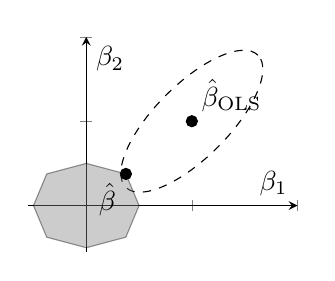
\begin{tikzpicture}
\begin{axis}[
    xlabel = \(\beta_1\),
    ylabel = \(\beta_2\),
    ymin = -1.1,
    ymax = 4,
    xmin = -1.1,
    xmax = 4,
    axis lines = center,
    yticklabels={,,},
    xticklabels={,,}
]

\draw[dashed, rotate around={45:(2,2)}] (2,2) ellipse (1.77 and 0.87);

\addplot[fill = gray, opacity = 0.4]
    coordinates {
    	(-1,0)
    	(-0.75, 0.75)
    	(0,1)
    	(0.75,0.75)
    	(1,0)
    	(0.75,-0.75)
    	(0,-1)
    	(-0.75,-0.75)
    	(-1,0)
    };
\addplot [only marks, mark=*] coordinates {(2,2)};
\node [above right,black] at (2,2) {\(\hat\beta_\text{OLS}\)};

\addplot [only marks, mark=*] coordinates { (0.75,0.75) };
\node [below left] at (0.75,0.75) {$\hat\beta$};
\end{axis}
\end{tikzpicture}   
        \end{column}
    \end{columns}
\end{frame}

\section{Wrap-Up}

\begin{frame}{Wrap-Up}
    
\end{frame}

% \begin{frame}[allowframebreaks]{References}
%   \bibliographytrue
%   \printbibliography[heading=none]
% \end{frame}

\end{document}
